\section{Ejercicio 6}


\subsection{Desarrollo}
Ejecutamos el lote anterior con el scheduler FCFS
 y lo comparamos con el ejercicio anterior con un solo procesador.\par
En un scheduler FCFS (primero en llegar, primero en ser servido), el órden de prioridad de los proceso se manejan como una cola FIFO: se asigna el procesador, al proceso que llegue primero. En este algoritmo de scheduling, el proceso utiliza la CPU hasta completarse.\par
El algoritmo de scheduling de RR (Round Robin), es similar a FCFS en el sentido que maneja una cola FIFO, pero cada proceso tiene un período de tiempo que, una vez agotado, indica la scheduler desalojar la tarea y correr la siguiente, la tarea desalojada pasa al final de la cola en estado de "espera" hasta que vuelve a ser su turno para obtener el procesador. La gran diferencia entre un algoritmo FCFS y uno RR está justamente en éste último tine un mecanismo de desalojo y el primero no.


\subsection{Experimentación}
Podemos ver que el gráfico de Gantt para el lote de tareas loteEj5.tsk de la figura \ref{fig:ej6FCFS} se asemeja mucho a la corrida del lote en \verb|SchedRR| con quantum 50, pues las tareas intensas de CPU tienen un tiempo total de corrida (51 ciclos) casi tan grande como el quantum que se les asigna, y en RR, no son desalojadas las tareas hasta que no se les agota el quantum.  Volcamos los datos de tiempo en la tabla \ref{tab:ej6FCFS} de tiempos para cada tarea\par
\begin{figure}[H]
  \centering
    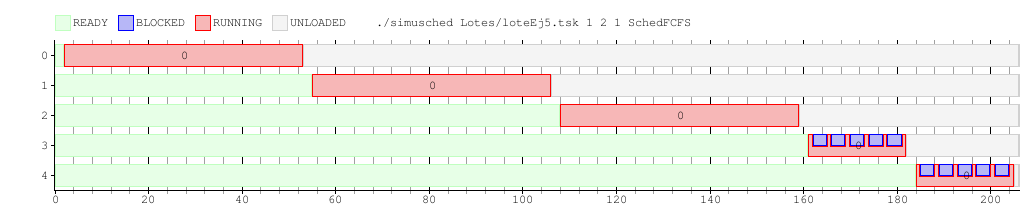
\includegraphics[width=1.1\textwidth]{imagenes/Ej6.png}
  \caption{loteEj5.tsk con FCFS}
  \label{fig:ej6FCFS}
\end{figure}


\begin{table}
\centering
\begin{tabular}{ | c | c | c | c | c | c | c | }
  \hline			
  pid & ciclos & inicio & fin & latencia & waiting time & tiempo total  \\
  \hline
0 & 51 & 0 & 53 & 2 & 2 & 53\\
1 & 51 & 0 & 106 & 55 & 55 & 106\\
2 & 51 & 0 & 159 & 108 & 108 & 159\\
3 & 21 & 0 & 182 & 161 & 161 & 182\\
4 & 21 & 0 & 205 & 184 & 184 & 205\\
  \hline
promedio & - & - & - & 102 & TaskCPU: 55  & TaskCPU: 106 \\
                & &  &  &  & TaskConsola: 172.5  & TaskConsola: 193\\
\hline
\end{tabular}
\caption{Tiempos para loteEj5.tsk con FCFS}\label{tab:ej6FCFS}
\end{table}

FCFS y RR con quantum 50 tienen latencia promedio similares, y waiting times y tiempos totales similares también para los preceso de E/S, pues en ambos casos, corren últimos y luego de que hayan corrido los proceso más largo de CPU. En cambio para las tareas intensas de CPU, éstos dos últimos valores son mejores en FCFS, justamente porque éstos procesos corren primeros y completos antes de cambiar a las tareas de E/S.\par